% "{'classe':('PSI'),'chapitre':'stat_frot','type':('application'),'titre':'Poulie-courroie', 'source':'Lycée Mistral -- Avignon.','comp':('B2-14','C1-05','C2-07'),'corrige':True}"
%\setchapterimage{fig_00.jpg}
\chapter*{Application \arabic{cptApplication} \\ 
Frottement exponentiel -- Poulie-courroie  \ifnormal $\star$ \else \fi \ifdifficile $\star\star$ \else \fi \iftdifficile $\star\star\star$ \else \fi -- \ifprof Corrigé \else Sujet \fi}
\addcontentsline{toc}{section}{Application \arabic{cptApplication} : Frottement exponentiel -- Poulie-courroie  \ifnormal $\star$ \else \fi \ifdifficile $\star\star$ \else \fi \iftdifficile $\star\star\star$ \else \fi -- \ifprof Corrigé \else Sujet \fi}

\iflivret \stepcounter{cptApplication} \else
\ifprof  \stepcounter{cptApplication} \else \fi
\fi

\setcounter{question}{0}
\marginnote{Lycée Mistral -- Avignon.}
\marginnote[1cm]{
\UPSTIcompetence[2]{B2-14}
\UPSTIcompetence[2]{C1-05}
\UPSTIcompetence[2]{C2-07}
}

Le problème du frottement d'une corde, d'une sangle ou d'une courroie sur une poulie ou
un tambour est un problème classique. 
\begin{obj}
Modéliser l'évolution de la tension dans un câble en fonction de l'angle d'enroulement sur une poulie. 
\end{obj}

On note $f$ le coefficient de frottement entre le câble et la poulie. 
\begin{center}
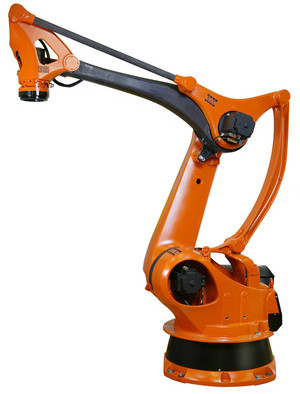
\includegraphics[width=.75\linewidth]{fig_01}
%\textit{}
\end{center}

On considère que le câble est enroulé d'un angle $\alpha$ autour de la poulie. Le câble est à la limite du glissement sous l'action des deux brins $\vect{T_1}$ et $\vect{T_2}$. Soit $M(\theta)$ un point de l'enroulement. 

\question{Après avoir isolé une tranche élémentaire de câble en $M(\theta)$ de largeur $\dd \theta$, réaliser un bilan des actions mécaniques extérieures. }
\ifprof
\begin{corrige}
BAME :
\begin{itemize}
\item action de tension du câble 1 $\vect{F}\left(\theta+\dfrac{\dd \theta}{2}\right)$;
\item action de tension du câble 2 $\vect{F}\left(\theta-\dfrac{\dd \theta}{2}\right)$;
\item action de la poulie sur le câble : $N\vect{u_r}+T\vect{u_{\theta}}$ avec $T=\pm fN$.
\end{itemize}

\end{corrige}
\else
\fi


\question{Appliquer le théorème en résultante statique en projection dans la base $\left( \vect{u_r}, \vect{u_{\theta}}\right)$.}
\ifprof
\begin{corrige}
L'application du TRS à la tranche de câble, on a $\vect{F}\left(\theta+\dfrac{\dd \theta}{2}\right) + \vect{F}\left(\theta-\dfrac{\dd \theta}{2}\right) + N\vect{u_r}+T\vect{u_{\theta}} = \vect{0}$.

En projetant dans $\left( \vect{u_r}, \vect{u_{\theta}}\right)$ on a :
 
$\left\{ 
\begin{array}{l}
-F\left(\theta+\dfrac{\dd \theta}{2}\right)  \sin\left(\dfrac{\dd \theta}{2}\right)  -F\left(\theta-\dfrac{\dd \theta}{2}\right) \sin\left(\dfrac{\dd \theta}{2}\right) + N= 0 \\
F\left(\theta+\dfrac{\dd \theta}{2}\right) \cos\left(\dfrac{\dd \theta}{2}\right) -F\left(\theta-\dfrac{\dd \theta}{2}\right) \cos\left(\dfrac{\dd \theta}{2}\right) + T = 0
\end{array}
\right.$.

\end{corrige}
\else
\fi


\question{En considérant que l'angle $\theta$ est petit, établir l'équation différentielle liant $f$ et $F(\theta)$ et $\theta$.}
\ifprof
\begin{corrige} ~\\
En utilisant $\cos \dd \theta/2 \simeq 1$ et $\sin \dd \theta/2 \simeq \dd \theta/2$ :
$\left\{ 
\begin{array}{l}
-F\left(\theta+\dfrac{\dd \theta}{2}\right)\dfrac{\dd \theta}{2} -F\left(\theta-\dfrac{\dd \theta}{2}\right) \dfrac{\dd \theta}{2} + N= 0 \\
F\left(\theta+\dfrac{\dd \theta}{2}\right) -F\left(\theta-\dfrac{\dd \theta}{2}\right) + T = 0
\end{array}
\right.$.


$
\Leftrightarrow \left\{ 
\begin{array}{l}
-\left(F\left(\theta+\dfrac{\dd \theta}{2}\right) +F\left(\theta-\dfrac{\dd \theta}{2}\right)\right) \dfrac{\dd \theta}{2} + N= 0 \\
F\left(\theta+\dfrac{\dd \theta}{2}\right) -F\left(\theta-\dfrac{\dd \theta}{2}\right) + T = 0
\end{array}
\right.$.

De plus, en faisant un DL à l'ordre 2, $F\left(\theta+\dfrac{\dd \theta}{2}\right)\simeq  F(\theta)+\dfrac{\dd \theta}{2} \dfrac{\dd F(\theta)}{\dd \theta}$.
On a donc : 
$
\left\{ 
\begin{array}{l}
-2 F\left(\theta\right) \dfrac{\dd \theta}{2} + N= 0 \\
 \dd F(\theta)+ T = 0
\end{array}
\right.$.

En utilisant le modèle de Coulomb, $T=\pm fN$

 $ \dd F(\theta)\pm f \left( 2 F\left(\theta\right) \dfrac{\dd \theta}{2}\right) = 0$
 $  \Leftrightarrow \dd F(\theta)\pm f  F\left(\theta\right) \dd \theta = 0$

%
%En utilisant le modèle de Coulomb, on a $T=fN$ et 
%
%$F\left(\theta+\dfrac{\dd \theta}{2}\right) -F\left(\theta-\dfrac{\dd \theta}{2}\right)  = -f \left(F\left(\theta+\dfrac{\dd \theta}{2}\right)\dfrac{\dd \theta}{2} +F\left(\theta-\dfrac{\dd \theta}{2}\right) \dfrac{\dd \theta}{2} \right)$.
%
%
%$ \Leftrightarrow F\left(\theta+\dfrac{\dd \theta}{2}\right) -F\left(\theta-\dfrac{\dd \theta}{2}\right)  + f \left(F\left(\theta+\dfrac{\dd \theta}{2}\right)\dfrac{\dd \theta}{2} +F\left(\theta-\dfrac{\dd \theta}{2}\right) \dfrac{\dd \theta}{2} \right) = 0$.
%
%$ \Leftrightarrow F\left(\theta+\dfrac{\dd \theta}{2}\right) \left(1 +f\dfrac{\dd \theta}{2} \right) -F\left(\theta-\dfrac{\dd \theta}{2}\right) \left(1+ f\dfrac{\dd \theta}{2} \right) = 0$.
%
%
%$ \Leftrightarrow  \left(1 +f\dfrac{\dd \theta}{2} \right)\left(F\left(\theta+\dfrac{\dd \theta}{2}\right) - F\left(\theta-\dfrac{\dd \theta}{2}\right) \right)  = 0$.
%
%En réutilisant l'hypothèse des petits angles, on a : 
%$ \Leftrightarrow  \left(1 +f\dfrac{\dd \theta}{2} \right)\left(F\left(\theta\right) - F\left(\theta\right) \right)  = 0$.

\end{corrige}
\else
\fi

\ifprof
\else
\begin{marginfigure}
\centering

\includegraphics[width=3cm]{Cy_11_Ch_02_Application_01_Poulie_qr}
\end{marginfigure}
\fi


\question{Résoudre l'équation différentielle pour établir la relation entre $T_1$, $T_2$, $f$ et~$\alpha$.}
\ifprof
\begin{corrige}
On a :
 $ \dd F(\theta)= \pm  F\left(\theta\right) \dd \theta $
  $ \Leftrightarrow \dfrac{ \dd F(\theta)}{ F\left(\theta\right)}= \pm \dd \theta $
  
  En intégrant l'équation précédente, on a :
  $\left[ \ln F \right] _{T_1}^{T_2} =\pm f \left[ \theta \right] _{0}^{\alpha}$
  Soit $\ln T_2 - \ln T_1 = -f\alpha$ $\Leftrightarrow \ln \dfrac{T_2}{T_1} = \pm f\alpha$ et $T_2 = T_1 \text{e}^{\pm f\alpha}$.
  
(Le signe dépend du sens de glissement. )
\end{corrige}
\else
\fi

